\section{Aufgabe 2} \label{ex2}
Die Aufgabe 2 wurde in zwei Unteraufgaben geteilt. Zuerst wurde mittels einer automatisch generierten 
Testfunktion im SDK und auf dem Zedboard geprüft, ob der selbst erstellte IP Core voll funktionsfähig ist. 
Erst danach wurde ein eigenes LED Muster geschrieben.

\subsection{Test des IP Cores}
Nach Konfiguration eines eigenen AXI GPIO IP Cores wurde zuerst die automatisch generierte Funktion: KES\_LAB2\_8BIT\_AXI\_Reg\_SelfTest ausgeführt.\\

C-Code des Aufrufes
\begin{verbatim}
  #include <stdio.h>
  #include "platform.h"
  #include "xil_printf.h"
  #include "kes_lab2_8bit_axi.h"

  #define BASE_ADDR XPAR_KES_LAB2_8BIT_AXI_0_S00_AXI_BASEADDR // 0x43C00000

  int main()  {
      init_platform();
      XStatus status = KES_LAB2_8BIT_AXI_Reg_SelfTest( (void *) BASE_ADDR);
      cleanup_platform();
      return 0;
  }
\end{verbatim}

Die automatisch generierte Test Funktion in kes\_lab2\_8bit\_axi\_selftest.c.
\begin{verbatim}
  /***************************** Include Files ***********************/
  #include "kes_lab2_8bit_axi.h"
  #include "xparameters.h"
  #include "stdio.h"
  #include "xil_io.h"

  /************************** Constant Definitions ********************/
  #define READ_WRITE_MUL_FACTOR 0x10

  XStatus KES_LAB2_8BIT_AXI_Reg_SelfTest(void * baseaddr_p) {
    u32 baseaddr;
    int write_loop_index;
    int read_loop_index;
    int Index;
    baseaddr = (u32) baseaddr_p;
    xil_printf("******************************\n\r");
    xil_printf("* User Peripheral Self Test\n\r");
    xil_printf("******************************\n\n\r");
    /*
     * Write to user logic slave module register(s) and read back
     */
    xil_printf("User logic slave module test...\n\r");

    for (write_loop_index = 0 ; write_loop_index < 4; write_loop_index++)
      KES_LAB2_8BIT_AXI_mWriteReg (baseaddr, write_loop_index*4,
            (write_loop_index+1)*READ_WRITE_MUL_FACTOR);
    for (read_loop_index = 0 ; read_loop_index < 4; read_loop_index++)
       if ( KES_LAB2_8BIT_AXI_mReadReg (baseaddr, read_loop_index*4) !=
            (read_loop_index+1)*READ_WRITE_MUL_FACTOR)
       {     
            xil_printf ("Error reading register value at address %x\n", 
                  (int)baseaddr + read_loop_index*4);
            return XST_FAILURE;
      }

    xil_printf("   - slave register write/read passed\n\n\r");
    return XST_SUCCESS;
  }
\end{verbatim}

\begin{minipage}{\textwidth}
    \begin{center}        
        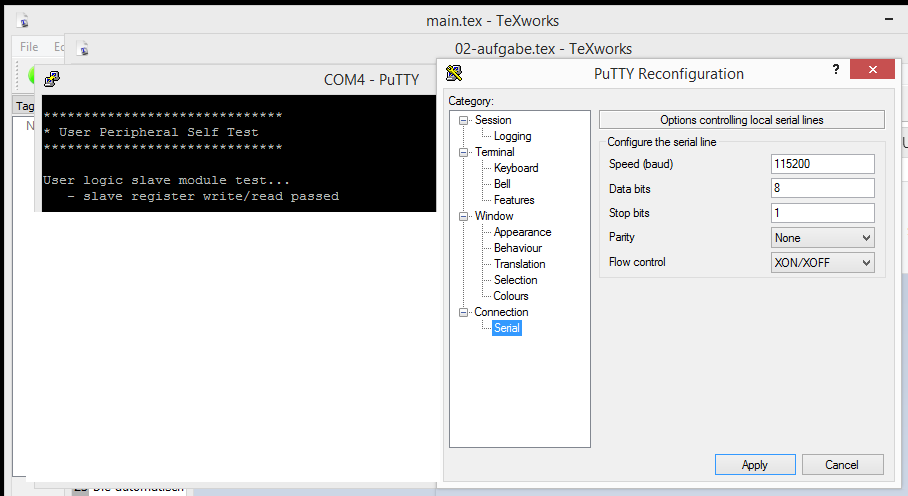
\includegraphics[scale=0.5]{img/debugselftest.png} 
    \end{center}
\end{minipage}
\begin{center}
Standard Debug Ausgabe
\end{center}

Oder als Alternative mit Rücklesen der geschriebenen Daten:
\begin{verbatim}
  for (read_loop_index = 0 ; read_loop_index < 4; read_loop_index++)
    if ( KES_LAB2_8BIT_AXI_mReadReg (baseaddr, read_loop_index*4) !=
      (read_loop_index+1)*READ_WRITE_MUL_FACTOR)
     {
        xil_printf ("Error reading register value at address %x\n", 
                           (int)baseaddr + read_loop_index*4);
        return XST_FAILURE;
     } else
        xil_printf ("Reading register value at address %x value %x\n\r",
            (int)baseaddr + read_loop_index*4, 
                  (read_loop_index+1)*READ_WRITE_MUL_FACTOR );
\end{verbatim}

\begin{minipage}{\textwidth}
    \begin{center}        
        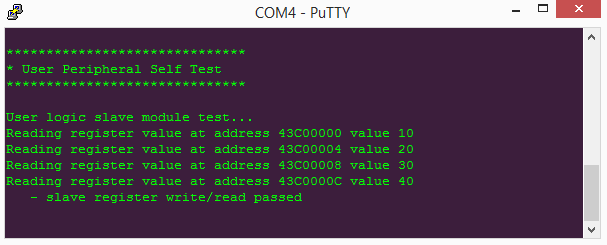
\includegraphics[scale=0.5]{img/debugselftest2.png} 
    \end{center}
\end{minipage}
\begin{center}
Logausgabe mit gelesenen Daten
\end{center}

\subsection{Aufgabe 2 Anzeige auf den LEDs über den IP Core}
Implementiert wurde eine laufende LED die schnell von LED 0 jeweils nach sehr kurzer Wartezeit auf die links 
liegende LED weitergeschaltet wird. Damit entsteht der Eindruck einer wandernden LED. Nach beenden eines 
Zyklus wird erneut gestartet.

\begin{verbatim}
  #include <stdio.h>
  #include "platform.h"
  //#include "xil_printf.h" 
  #include "kes_lab2_8bit_axi.h"
  //#include "xparameters.h"
  #include "xil_io.h"

  #define BASE_ADDR XPAR_KES_LAB2_8BIT_AXI_0_S00_AXI_BASEADDR // 0x43C00000
  #define LED_DELAY  40000000

  int main()
  {
    init_platform();

    int i, delay;
    uint pattern = 1;

    while (1) {
      for ( i = 0; i <= 8; i++ ) {
        KES_LAB2_8BIT_AXI_mWriteReg ((u32)BASE_ADDR, 0, pattern);
        pattern <<= 1;
        for ( delay = 0;  delay  < LED_DELAY; delay++ );
    }
    pattern = 1;
  }
  cleanup_platform();
  return 0;
}
\end{verbatim}



\subsection{VHDL}

\textbf{Funktion der Pfeile in Zuweisungen  <=, =>}\\
<= is an assignment - specifically a signal assignment, driving a signal with a value from somewhere else. For a physical analogy, the thing on the right hand side drives a value onto the left hand side.\\

=> is a port mapping from a pin to a signal. This is not an assignment - the physical analogy might be soldering a pin to a wire.\\

You can only do "soldering" to instantiations, so => mapping only happens inside a port map. And there, "pins" always go on the left (because that's what the language rules say), which is why you can't do x <= port\_a in a port map.\\

Signal assignments go from right to left using <=. The right side must be an input signal from the entity or a signal declared in a process. The left side can be an output signal (or input/buffer) from the entity, a signal declared in the process or a variable declared in the process.\\

Beside port mapping mentioned in other answers, the => arrow is also used for a totally different thing - to construct vectors. For example, if v is a 4 bit vector, then v <= (others => '0') will assign "0000" to v. The ``=>` within the parentheses is a shortcut for assigning different values in different places inside the vector.\\




